\section{ANALISIS E INTERPRETACION DE RESULTADOS} 
-Al compilar el proyecto de prueba, las pruebas aparecen en el Explorador de pruebas. Si el Explorador de pruebas no está visible, elija Prueba en el menú de Visual Studio, elija Ventanas y, después, Explorador de pruebas.
-Se puede elegir Ejecutar todas para ejecutar todas las pruebas o bien Ejecutar para elegir un subconjunto de pruebas que se desea ejecutar. Después de ejecutar un conjunto de pruebas, aparecerá un resumen de la serie de pruebas en la parte inferior de la ventana Explorador de pruebas. Seleccione una prueba para ver los detalles de esa prueba en el panel inferior. 
\begin{itemize}
	\item Al compilar el proyecto de prueba.
	\begin{figure}[htb]
\begin{center}
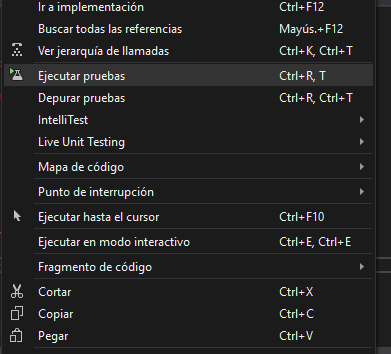
\includegraphics[width=12cm]{./Imagenes/1-11}
\end{center}
\end{figure}
	\item Explorador de pruebas.
\begin{figure}[htb]
\begin{center}
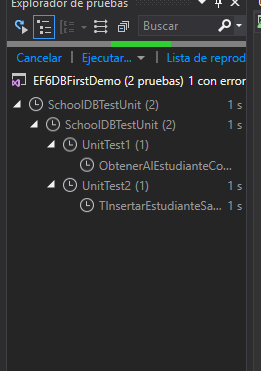
\includegraphics[width=12cm]{./Imagenes/1-12}
\end{center}
\end{figure}
\end{itemize}
